\chapter{Architecture and Design}

\epigraph{In general, when modeling phenomena in science and
  engineering, we begin with simplified, incomplete models. As we
  examine things in greater detail, these simple models become
  inadequate and must be replaced by more refined
  models.}{\textit{Structure and Interpretation of Computer Programs,
    Section 1.1.5}\cite{sicp}}

\section{Structure of combox}

combox consists of two main components -- the combox directory and the
node directories. The combox directory is the place where the user
stores all her files; the node directories are the directories under
which encrypted shards of the files (in the combox directory) are
scattered to. A node directory is the file storage provider's
directory, for instance, the Dropbox directory and the Google Drive
directory are node directories.

When a file \verb+file.ext+ is created in the combox directory, combox
splits the \verb+file.ext+ into \verb+N+ shards, where \verb+N+ is the
number of node directories; if there are two node directories (Dropbox
directory and Google Drive driver), then 2 shards are created. Each
shard of the file is then encrypted and the encrypted shards are
spread evenly across the node directories; if there are two node
directories -- Dropbox directory and Google Drive directory -- combox
will create two encrypted shards of file \verb+file.ext+ --
\verb+file.ext.shard0+, \verb+file.ext.shard1+ -- and place one
encrypted shard under the Dropbox directory and the other encrypted
shard under the Google Drive directory. Now, the Dropbox client and
the Google client will sync the respective shards that was place under
their directories to their servers.

\begin{figure}[h]
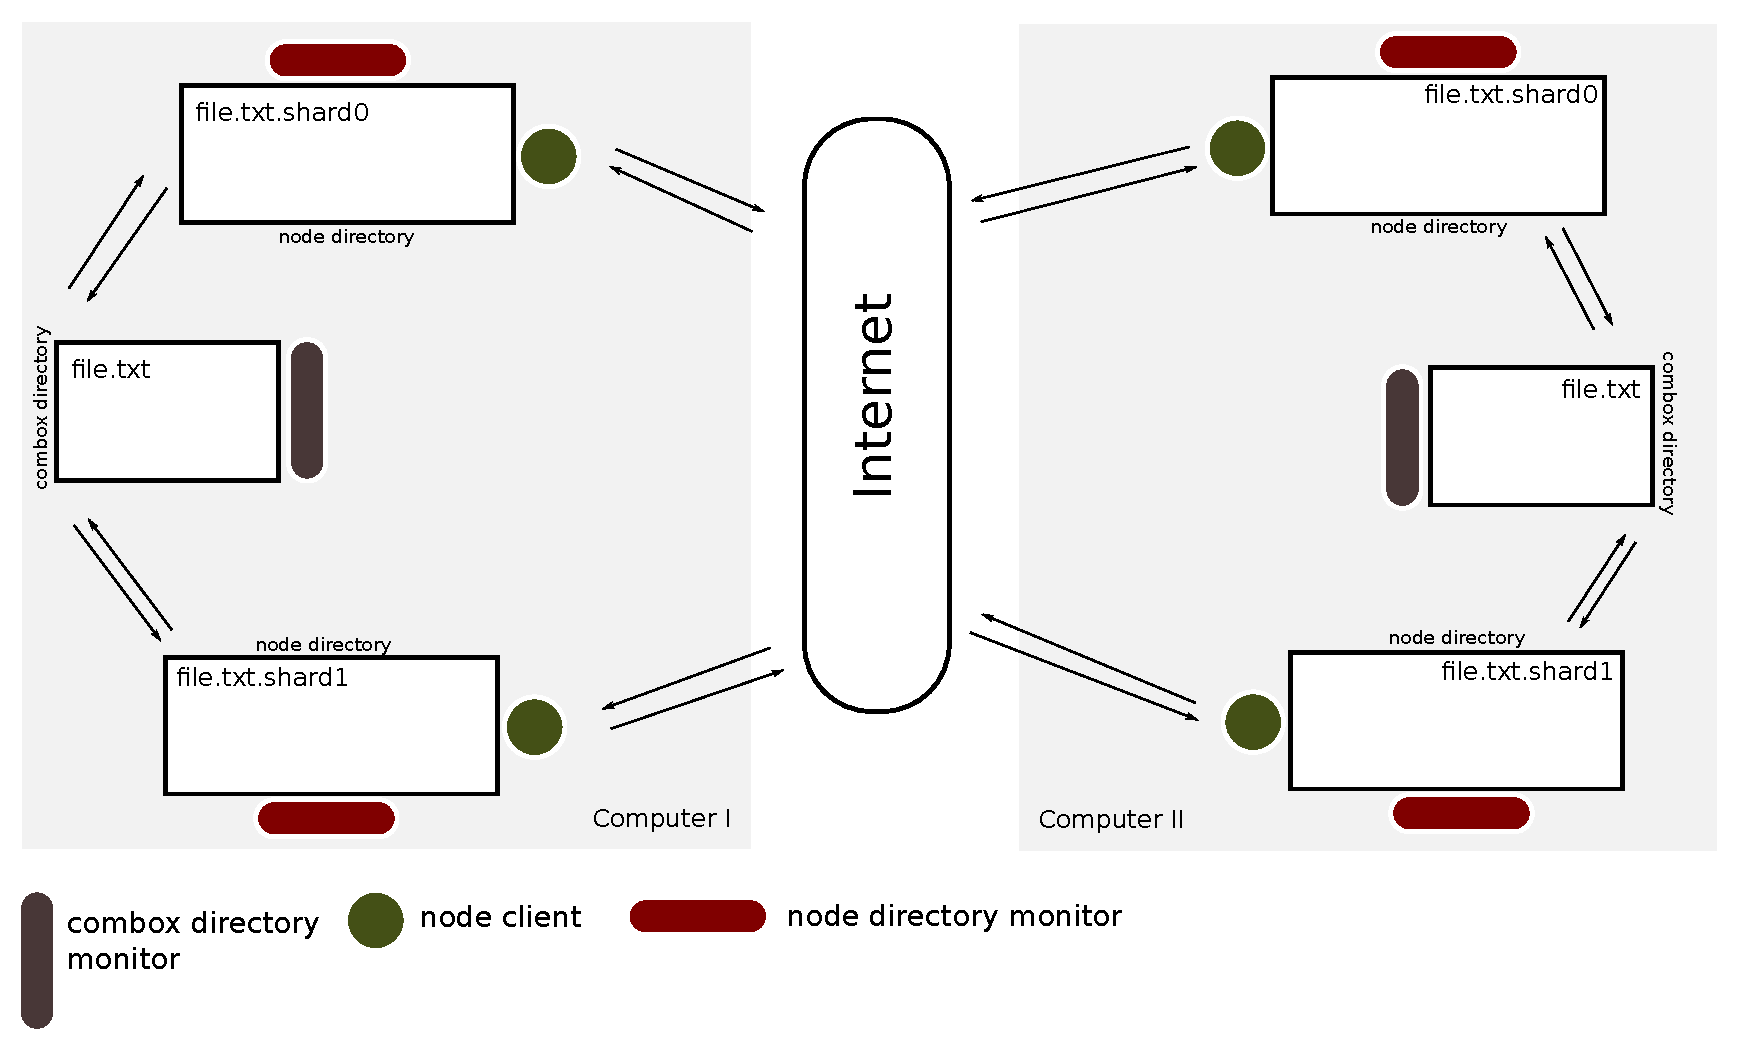
\includegraphics[scale=0.6]{4-combox-structure}
\caption{High level view of combox on two computers.}
\label{fig:4-combox-structure}
\end{figure}

Now, we can move to another computer and start combox on it. First,
the node clients (Dropbox client and the Google Drive client) will
sync the new encrypted shards to their respective directories. Once
the encrypted shards are synced to the node directories, combox will
pick the encrypted shards -- \verb+file.ext.shard0+,
\verb+file.ext.shard1+ -- decrypt them and reconstruct into
\verb+file.ext+ and place in the respective location under the combox
directory; figure \ref{fig:4-combox-structure} illustrates this. The
process is similar for file modification, deletion and rename/move.

\subsection{combox configuration}\label{sec:4-combox-config}

combox configuration triggers automatically when combox finds that it
is not configured on this computer. The combox configuration setups up
the combox directory; asks the user to point to the location of the
node directories; reads the key (passphrase) to be used to encrypt
file shards that are spread across the node directories. The combox
configuration is written to
\verb+$HOME/.combox/config.yaml+; this YAML configuration file can be
manually edited by the user.

The \verb+config_cb+ function in the \verb+combox.config+ module is
responsible for carrying out the combox configuration. Prior to
version \verb+0.2.0+, the combox configuration was purely done through
the CLI, from \verb+0.2.0+ onwards, be default, the combox
configuration done through a graphical interface; it is still possible
to configure combox through the CLI with the \verb+--cli+ switch.

A demo of combox configuration using the graphical interface on
GNU/Linux can be viewed at
\url{https://ricketyspace.net/combox/combox-config-gui-glued-gnu.webm};
the same demo of combox configuration using the graphical interface on
OS X can be viewed at
\url{https://ricketyspace.net/combox/combox-config-gui-glued-osx.webm}.

\subsection{combox directory monitor}\label{sec:4-combox-cdirm}

combox directory monitor is an instance of
\verb+combox.events.ComboxDirMonitor+ monitoring the combox directory
for changes. When changes are made to the combox directory, the combox
directory monitor is responsible for correctly detecting the type of
change and doing the right thing at that instance of time.

When a file is created in the combox directory, the combox directory
monitor will take that file, split it into \verb+N+ (equal to the
number of node directories) shards, encrypt the shards, spread the
encrypted shards to the node directories, and finally store the hash
of the file in the local combox database.

When a file is modified in the combox directory, the combox directory
monitor will take that modified file, split it into \verb+N+ (equal to
the number of node directories) shards, encrypt the shards, spread the
encrypted shards to the node directories, and finally update the hash
of the file in the local combox database.

When a file is deleted in the combox directory, the combox directory
monitor will remove the encrypted shards of the file in the node
directories and get rid of the file's hash from the local combox
database.

When a file is moved/renamed in the combox directory, the combox
directory monitor will move/rename encrypted in the node directories,
the file's hash from the local combox database and store the hash of
file under its new name.

\subsection{Node directory monitor}\label{sec:4-combox-nodirm}

Node directory monitor is an instance of
\verb+combox.events.NodeDirMonitor+ monitoring a node directory. When
changes are made to the node directory, the node directory monitor is
responsible for correctly detecting the type of change and doing the
right thing at that instance of time. Each node directory has a
dedicated node directory monitor; if there are 2 node directories,
then combox will instantiate 2 node directory monitors.

When an encrypted shard is created in the node directory due to a file
created on another computer, the node directory first checks if the
respective file' encrypted shard(s) has/have arrived in other node
directory/directories. If all encrypted shards have arrived, then the
node directory takes all the encrypted shards, decrypts them,
reconstructs the file and creates the file in the combox directory of
this computer and stores the hash of the newly created file in the
local combox database. If the all the encrypted shards have not
arrived, then the node directory does not do anything. It must be
observed here that the node directory monitor of the last node
directory which gets the encrypted shard will be the one to perform
the file reconstruction and creation.

When an encrypted shard is modified in the node directory due to a
file modified on another computer, the node directory first checks if
the respective file' modified encrypted shard(s) has/have arrived in
other node directory/directories. If all modified encrypted shards
have arrived, then the node directory takes all the modified encrypted
shards, decrypts them, reconstructs the file and puts the modified
version of the file in the combox directory of this computer and
updates the file's hash in the local combox database. If the all the
modified encrypted shards have not arrived, then the node directory
does not do anything. It must be observed here that the node directory
monitor of the last node directory which gets the modified encrypted
shard will be the one to perform the file reconstruction and will place
the modified file in the combox directory.

When an encrypted shard is deleted in the node directory due to a file
deleted on another computer, the node directory first checks if the
respective file' encrypted shard(s) has/have been deleted in other
node directory/directories. If all encrypted shards have been deleted
from the node directories, then the node directory deletes the file in
the combox directory of this computer and removes its information from
the local combox database. If all encrypted shards have not been
deleted, then the node directory does not do anything. It must be
observed here that the node directory monitor of the last node
directory in which the encrypted shard is deleted will be the one to
delete the file from the combox directory.

When an encrypted shard is moved/renamed in the node directory due to
a file moved/renamed on another computer, the node directory first
checks if the respective file' moved/renamed encrypted shard(s)
has/have arrived in other node directory/directories. If all
moved/renamed encrypted shards have arrived, then the node directory
takes all the moved/renamed encrypted shards, decrypts them,
reconstructs the moved/renamed file and puts the moved/renamed the file
in the combox directory of this computer and stores the hash under the
file' new name in the local combox database. If the all the
moved/renamed encrypted shards have not arrived, then the node
directory does not do anything. It must be observed here that the node
directory monitor of the last node directory which gets the
moved/renamed encrypted shard will be the one to perform the file
reconstruction and will place the moved/renamed file in the combox
directory.

\subsection{Database structure}\label{sec:4-combox-db}

To keep it simple, stupid, I decide to maintain bare minimum
information about files, stored in the combox directory, and depend on
file system events to do the right thing when changes takes place in
the combox directory.

The only information that is stored in the database, about a file in
the combox directory is its SHA-512 hash; The SHA-512 hash of a file
is enough information to detect in the file. In the database, there
also four dictionaries -- \verb+file_moved+, \verb+file_deleted+,
\verb+file_created+, \verb+file_modified+ -- which tracks the number
of shards of a file that was moved/deleted/created/modified due the
respective file being moved/deleted/created/modified on another
computer; these four dictionaries are primarily used by the
\verb+NodeDirMonitor+ to detect remote file
movement/deletion/creation/modification and triggering file
reconstruction from shards at the right time.

The database is a JSON file on the disk, stored by default at
\verb+$HOME/.combox/silo.db+. The
\verb+combox.silo.ComboxSilo+\cite{combox-src:silo.ComboxSilo} is the
sole interface to read from and write to database. The database is
primarily accessed and modified by the combox directory monitor
(\verb+ComboxDirMonitor+) and the node directory monitor
(\verb+NodeDirMonitor+) through a shared Lock\cite{py:threading.Lock}
that ensures that only one entity\footnote{An entity can be the combox
  directory monitor or one of the node directory monitors} can
access/modify the database at a time.

Below is an illustration of the structure of the combox database:

\begin{verbatim}
{
  "/home/rsd/combox/ipsum.txt": "e3206df2bb2b3091103ab9d...",
  "/home/rsd/combox/tk-shot-osx.png": "7fcf1b44c15dd95e0...",
  "/home/rsd/combox/thgttg-21st.png": "0040eedfc3eeab546...",
  "/home/rsd/combox/lorem.txt": "5851dd7a4870ff165facb71...",
  "/home/rsd/combox/the-red-star.jpg": "4b818126d882e552...",
  "file_moved": {},
  "file_deleted": {},
  "file_created": {},
  "file_modified": {},
}
\end{verbatim}

The \verb+combox.silo.ComboxSilo+, which is the sole interface to read
from and write to the database, uses the pickleDB
library\cite{pylib:pickledb}. The pickleDB is a very basic key-value
store which allows one to store information in the JSON format; if I
would have not found this library or if this library was never by
Harrison Erd, I've would have written something very similar to this
library as part of combox to realize the basic key-value storage that
is needed to track the hashes of the files stored in the combox
directory.

It must be noted that the combox database stored on each computer is
independent and does not communicate or make transactions with the
combox databases located in other computers.

\section{combox modules overview}

combox is spread into modules that have functions and/or classes. As
of \verb+2016-02-04+ combox is considerably a small program:

\begin{verbatim}
$ wc -l combox/*.py
  144 combox/cbox.py
  178 combox/config.py
  241 combox/crypto.py
  891 combox/events.py
  541 combox/file.py
  454 combox/gui.py
    0 combox/__init__.py
   71 combox/log.py
  278 combox/silo.py
   29 combox/_version.py
 2827 total
\end{verbatim}

This section gives an overview of each of the combox modules with
extreme brevity:

\begin{description}
\item[combox.cbox] This module contains \verb+run_cb+ function runs
  combox; it creates an instance \verb+threading.Lock+ for database
  access and a shared \verb+threading.Lock+ for the
  \verb+combox.events.ComboxDirMonitor+ and
  \verb+combox.events.NodeDirMonitor+; it initializes an instance
  \verb+combox.events.ComboxDirMonitor+ that monitors the combox
  directory and an instance of \verb+combox.events.NodeDirMonitor+ for
  each node directory for monitoring the node directories. This
  modules also houses the \verb+main+ function that parses commandline
  arguments, starts combox configuration if needed or loads the combox
  configuration file to start running combox.
\item[combox.config] Accomodates two import functions --
  \verb+config_cb+ and \verb+get_nodedirs+. The \verb+config_cb+ is
  the combox configuration function that allows the user to configure
  combox; this function was designed in a such way that it was
  possible to use for both CLI and GUI methods of configuring
  combox. The \verb+get_nodedirs+ function returns, as a list, the
  paths of the node directories; this function use used in numerous
  places in other combox modules.
\item[combox.crypto] This has functions for encrypting and decrypting
  data; encrypting and decrypting shards (\verb+encrypt_shards+ and
  \verb+decrypt_shards+); a function for splitting a file into shards,
  encrypting those shards and spreading them across node directories
  (\verb+split_and_encrypt+); a function for decrypting the shards
  from the node directories, reconstructing the file from the
  decrypted shards and put the file back to the combox directory
  (\verb+decrypt_and_glue+). Functions \verb+split_and_encrypt+ and
  \verb+decrypt_and_glue+ are the two functions that that are
  extensively used by the \verb+combox.events+ module; all other
  functions in this module are pretty much helper functions are
  \verb+split_and_encrypt+ and \verb+decrypt_and_glue+ functions and
  are not used by other modules.
\item[combox.events] This module took the most time to write and test
  and it is the most complex module in combox at the time of writing
  this report. It contains just two classes -- \verb+ComboxDirMonitor+
  and \verb+NodeDirMonitor+. The \verb+ComboxDirMonitor+ inherits the
  \verb+watchdog.events.LoggingEventHandler+ and is responsible for
  monitoring for changes in the combox directory and doing the right
  thing when change happens in the combox directory. The
  \verb+NodeDirMonitor+ also inherits
  \verb+watchdog.events.LoggingEventHandler+ and similarly responsible
  for monitoring a node directory and doing the right thing when a
  change happens in the node directory; subjectively,
  \verb+NodeDirMonitor+ is slightly more complex than the
  \verb+ComboxDirMonitor+.
\item[combox.file] This is the second largest module in combox. It
  contains utility functions for reading, writing, moving
  files/directiores, hashing files, splitting a file into shards, glue
  shards into a file, manipulating directories inside combox and node
  directories.
\item[combox.gui] Contains the \verb+ComboxConfigDialog+ class; it is
  the graphical interface for configuring combox. The class uses the
  Tkinter library\cite{pylib:tkinter} for spawing graphical
  elements. Other graphical libraries include PyQt\cite{pylib:qt}
  were considered Tkinter was chosen over others because it works on
  all Unix systems and Microsoft's Windows and it is part of the core
  python (version 3).
\item[combox.log] All the messages to \verb+stdout+ and \verb+stderr+
  are sent through the functions \verb+log_i+ and \verb+log_e+
  functions defined in this module.
\item[combox.silo] Contains the \verb+ComboxSilo+ class which is the
  canonical interface for combox for managing information about the
  files in the combox directory. Internally, the \verb+ComboxSilo+
  class uses the pickleDB library\cite{pylib:pickledb}.
\item[combox.\_version] This is \emph{private} module that contains
  variables that contain the value of the present version and release
  of combox. The \verb+get_version+ function in this module returns
  the full version number; this function used by \verb+setup.py+.
\end{description}

\section{Language choice}

Back in October of 2014, I was learning to write in Python and when I
had to start working on combox, I chose to write combox in Python. In
my first commit to the combox repository, I had to say this about
Python:

\begin{verbatim}
commit 2def977472b2e77ee88c9177f2d03f12b0263eb0
Author: rsiddharth <rsiddharth@ninthfloor.org>
Date:   Wed Oct 29 23:24:58 2014 -0400

    Initial commit: File splitter & File gluer done.

    ...

    I like to write python FWIW. But after reading a dialect of Lisp when
    I come back to python, it does not look very beautiful. I guess I'm
    pretty convinced that there is no language that can ape the beauty of
    Lisp.
\end{verbatim}

If I were to write that commit message today (\verb+2016-02-04+), I
would've phrased my reflections about Python differently. While I've
not found a language that is as intrinsically beautiful as Lisp, I
think it is not quite right to compare Lisp and Python. Python is a
very readable language and it tends to be very accessible to
beginners. Also, it is hard to write unreadable Python code.

\section{DRY}

The core functionality of combox is to split, encrypt file shards,
spread them across node directories (Google Drive and Dropbox) and
decrypt, glue shards and put them back to the combox directory when a
file is created/modified/deleted/moved in another computer. The plan
was to use external libraries to accomplish things that fell outside
the realm of what I consider the ``core functionality of combox''; the
main reason behind this decision was to duly be an indolent programmer
and not indulge in trying to solve problems that others have already
solved.

The \verb+watchdog+\cite{pylib:watchdog} library was chosen for file
monitoring; this library is compatible with Unix systems and
Windows. The \verb+pycrypto+ library\cite{pylib:pycrypto} was used for
encrypting data; combox uses AES encryption scheme to encrypt file
shards. The \verb+pickleDB+\cite{pylib:pickledb} library was used to
store information about files in the combox directory; this library is
not very clean, but, it was what I exactly looking for, if there was
no \verb+pickleDB+, I would've most probably written something similar
to it and made it as part of combox.

Looking back, the decision to use external libraries reduced the
complexity of combox, reduced the time to complete the initial working
version of combox and made it possible to spend more than 3 months
just testing and fixing issues in combox.

\section{Operating system compatibility}\label{4-os-compat}

combox was developed on a GNU/Linux machine, a conscious effort was
made to write in an operating system independent way. The top criteria
for choosing a library to use in combox was that it had to be
compatible on \emph{all} of the three major computing platforms in
2014-2016\footnote{GNU/Linux, OS X and, Windows}.

As we were nearing the \verb+0.1.0+ release, combox was tested on OS X
(See chapter \ref{ch:5}) and OS X specific issues that were found
eventually were eventually fixed. The initial \verb+0.1.0+ release was
compatible with GNU/Linux and OS X.

After the initial release of combox, we wanted to see if combox would
be compatible with Windows. We found that:

\begin{itemize}
\item Setting up the parapharnalia to run combox was
  non-trivial\cite{doc:combox-setup-windoze}.
\item The unit tests for the \verb+combox.file+ module royally failed.
\end{itemize}

At the time of writing the report, combox is in version \verb+0.2.2+
and it still not compatible with Windows. Comprehensive documentation
of setting up the development environment for combox on Windows was
written\cite{doc:combox-setup-windoze} to make it less cumbersome for
anyone who would want to work on making combox compatible with
Windows.

\section{combox as a python package}\label{4-pypi}

Before version \verb+0.2.0+, the canonical way to install combox was
to pull the source from the \verb+git+ repository with:

\begin{verbatim}
  git clone git://ricketyspace.net/combox.git
\end{verbatim}

Then, do:

\begin{verbatim}
  cd combox
\end{verbatim}

Finally install combox with:

\begin{verbatim}
  python setup.py install
\end{verbatim}

Yes, installing combox on a machine was indeed non-trivial.

Python has a package registry called CheeseShop\footnote{code name for
  Python Package Index, see https://wiki.python.org/moin/CheeseShop};
all packages registered at the CheeseShop can be installed using
\verb+pip+ -- Python's platform independent package managment
system\cite{py:pip} -- with:

\begin{verbatim}
  pip install packagename
\end{verbatim}

To make it easier for (python) users to install combox on their
machine, an effort was made to make it a python
package\cite{py:package-guide}. From version \verb+0.2.0+, combox has
been registered python package at the CheeseShop. (Python) users can
now easily get a copy of combox on their machine with:

\begin{verbatim}
  pip install combox
\end{verbatim}

All versions of combox that is available through the CheeseShop are
digitally signed using the following GPG key:

\begin{verbatim}
pub   4096R/00B252AF 2014-09-08 [expires: 2017-09-07]
      Key fingerprint = C174 1162 CEED 5FE8 9954  A4B9 9DF9 7838 00B2 52AF
uid                  Siddharth Ravikumar (sravik) <sravik@bgsu.edu>
sub   4096R/09CECEDB 2014-09-08 [expires: 2017-09-07]
\end{verbatim}

All versions of combox's source are also available as a compressed
\verb+TAR+ ball and as a \verb+ZIP+ archive; they can be downloaded
from \url{https://ricketyspace.net/combox/releases.html}.

\section{With the benefit of hindsight}\label{4-hindsight}

combox's node monitor (\verb+combox.events.NodeDirMonitor+) was
written with the assumption that the node monitor will be the only
entity that will be making changes to the node directory that it is
monitoring. When started testing combox with node clients (Dropbox
client and Google Drive client), we observed that the node clients
made changes to the node directory when a file was
created/modified/renamed/deleted; for instance, when a shard, in the
Dropbox node directory, was modified on a remote computer, the Dropbox
client would first pull the newer version of the shard under the
\verb+.dropbox.cache+ directory as a temprorary file, move the older
version of the shard under \verb+.dropbox.cache+ as a backup, and
finally move the latest version of the shard, stored as a temprorary
file under the \verb+.dropbox.cache+ directory, to the respective
location in the Dropbox node directory; when a shard, in the Google
Drive node directory, was remotely modified on a remote computer, the
Google Drive client would delete the older version of the shard from
the Google Drive node directory and then create the newer version of
the shard in the respective location under the Google Drive node
directory. Since combox did not know about the node client's
behaviour, it confused combox and broke it royally; we had to make
major changes to the \verb+combox.eventns.NodeDirMonitor+ class to
make combox aware of the node client's behavior, this eventually
brutally obliterated the simplicity of the
\verb+combox.eventns.NodeDirMonitor+ class which I was proud of.

I'm not sure how I would have written the \verb+combox.events+ module
if I had known about the Dropbox and Google Drive client's behaviour
before writing the \verb+combox.events.NodeDirMonitor+ or the
\verb+combox.events.ComboxDirMonitor+ classes. Looking back, if there one
thing I would want to re-think/redo, it is the \verb+combox.events+
module.

The most important lesson I'm taking away from the experience of
writing combox is the insight of how easy it is to ruthless crush the
simplicity of a program due to unforeseen use cases.

\verb+<3+
